
\documentclass{standalone}
\usepackage[T1]{fontenc}
\usepackage[utf8]{inputenc}          % needed for French accents
\usepackage{pgfplotstable}
\usepackage{pgfplots}
\pgfplotsset{compat=1.18}
\usepackage{siunitx}                 % optional, nicer y‑axis numbers
\usepackage{booktabs}                % pretty tables for the optional preview

% -------------------------------------------------
% Helper that removes the internal \pgfpl@@ wrapper
% -------------------------------------------------

\begin{document}

    % This file was created with matplot2tikz v0.4.0.
    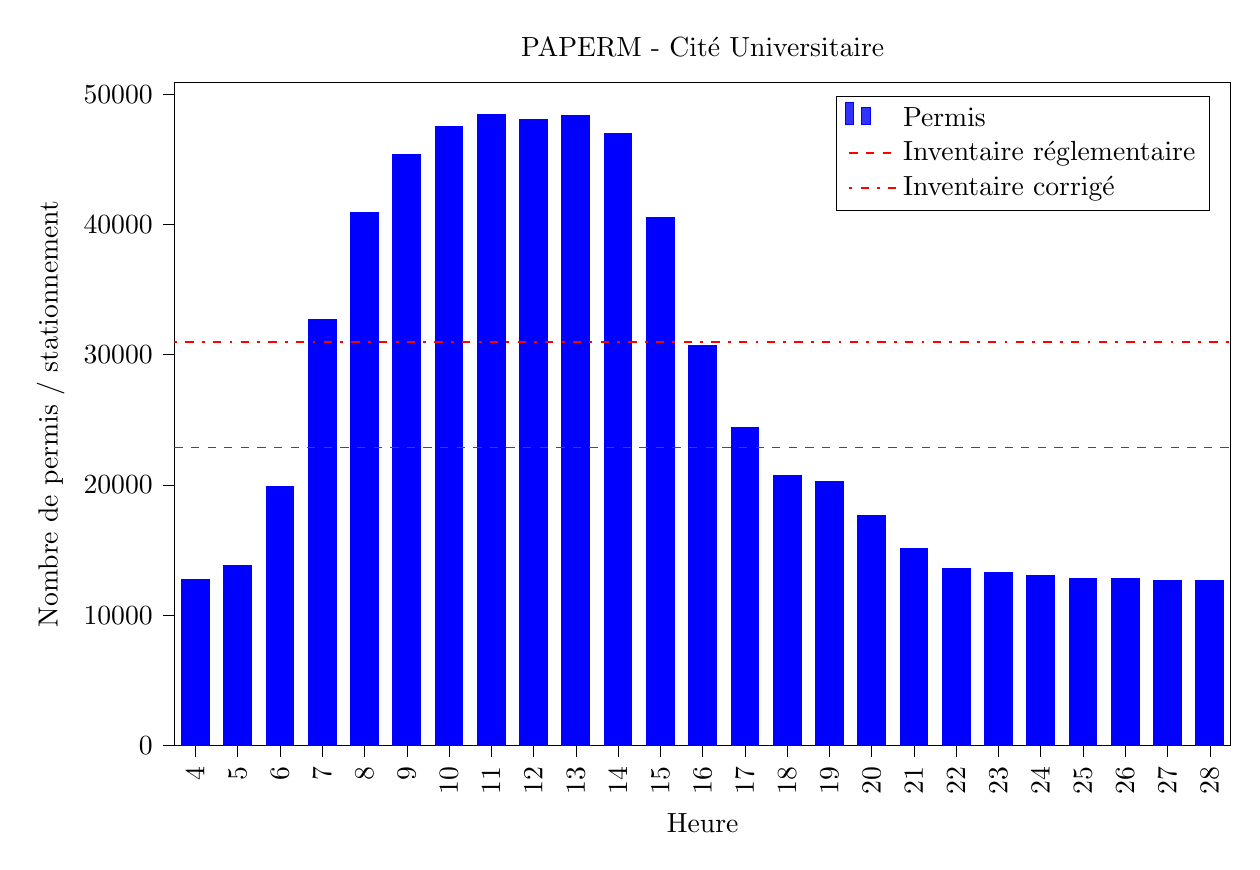
\begin{tikzpicture}
        \begin{axis}[
        height=10cm,
        legend cell align={left},
        legend style={fill opacity=0.8, draw opacity=1, text opacity=1},
        minor xtick={},
        minor ytick={},
        tick align=outside,
        tick pos=left,
        title={PAPERM - Cité Universitaire},
        width=15cm,
        xlabel={Heure},
        xmin=3.5, xmax=28.5,
        xtick style={color=black},
        xtick={0,1,2,3,4,5,6,7,8,9,10,11,12,13,14,15,16,17,18,19,20,21,22,23,24,25,26,27,28},
        xticklabel style={rotate=90.0},
        ylabel={Nombre de permis / stationnement},
        ymin=0, ymax=50898.75,
        ytick style={color=black},
        ytick={0,10000,20000,30000,40000,50000,60000},
        yticklabels={
          \(\displaystyle {0}\),
          \(\displaystyle {10000}\),
          \(\displaystyle {20000}\),
          \(\displaystyle {30000}\),
          \(\displaystyle {40000}\),
          \(\displaystyle {50000}\),
          \(\displaystyle {60000}\)
        },
        scaled ticks=false
        ]
        
        \addplot[ybar,draw=blue,fill=blue,legend image post style={/pgfplots/ybar legend}]
        coordinates{
            (4,12769)
            (5,13784)
            (6,19843)
            (7,32672)
            (8,40902)
            (9,45350)
            (10,47533)
            (11,48475)
            (12,48074)
            (13,48330)
            (14,46995)
            (15,40563)
            (16,30693)
            (17,24422)
            (18,20740)
            (19,20285)
            (20,17620)
            (21,15084)
            (22,13600)
            (23,13281)
            (24,13053)
            (25,12821)
            (26,12772)
            (27,12676)
            (28,12676)
        };
        
        \addlegendentry{Permis}
        \addplot [semithick, red, dashed]
            table {%
                3.5 22883
                28.5 22883
            };
        \addlegendentry{Inventaire réglementaire}
        \addplot [semithick, red, dash pattern=on 1pt off 3pt on 3pt off 3pt]
        table {%
        3.5 30976
        28.5 30976
        };
        \addlegendentry{Inventaire corrigé}
        \end{axis}
    
    \end{tikzpicture}

\end{document}